\documentclass[a4paper,12pt]{article}

% Pacotes essenciais
\usepackage[utf8]{inputenc}
\usepackage[T1]{fontenc}
\usepackage[brazil]{babel}
\usepackage{amsmath, amssymb}
\usepackage{graphicx}
\usepackage{booktabs}
\usepackage{caption}
\usepackage{siunitx}
\usepackage{geometry}
\geometry{a4paper, margin=1in}

\title{Relatório Detalhado (Atividades 5-6): \\ Redução de Dimensionalidade com PCA e seu Impacto}
\author{Lucas José Lemos Braz (Análise gerada por IA)}
\date{Agosto, 2025}

\begin{document}

\maketitle

\section{Introdução}

As Atividades 5 e 6 dão sequência à análise, abordando um dos passos mais importantes em pipelines de aprendizado de máquina para dados de alta dimensão: a \textbf{redução de dimensionalidade}. Tendo estabelecido um baseline de desempenho nos espaços de pixels original (A1-2) e rotacionado (A3-4), o foco agora se volta para a compressão da informação.

O processo foi dividido em duas etapas:
\begin{enumerate}
    \item \textbf{Atividade 5:} Análise quantitativa e qualitativa dos componentes principais para determinar a dimensionalidade intrínseca dos dados, ou seja, o número de componentes (\(q\)) necessário para reter 98\% da variância original.
    \item \textbf{Atividade 6:} Avaliação do desempenho e do custo computacional dos classificadores no subespaço de baixa dimensão (\(q \ll d\)) encontrado na etapa anterior.
\end{enumerate}
O objetivo é verificar se a compressão, além de gerar ganhos de eficiência, pode manter ou até melhorar a acurácia dos modelos ao atuar como um filtro de ruído.

\section{Atividade 5: Análise de Componentes Principais}

Esta atividade é exploratória e busca responder à pergunta: quão redundante é a informação contida nos 900 pixels de cada imagem de face?

\subsection{Análise Quantitativa: Variância Explicada}

Para determinar a dimensionalidade \(q\), um modelo PCA foi ajustado sobre o conjunto de treino completo. A partir dos autovalores da matriz de covariância, calculou-se a variância explicada acumulada por um número crescente de componentes principais. O critério, conforme o enunciado, era encontrar o menor \(q\) que retivesse pelo menos 98\% da variância total.

\begin{figure}[h!]
  \centering
  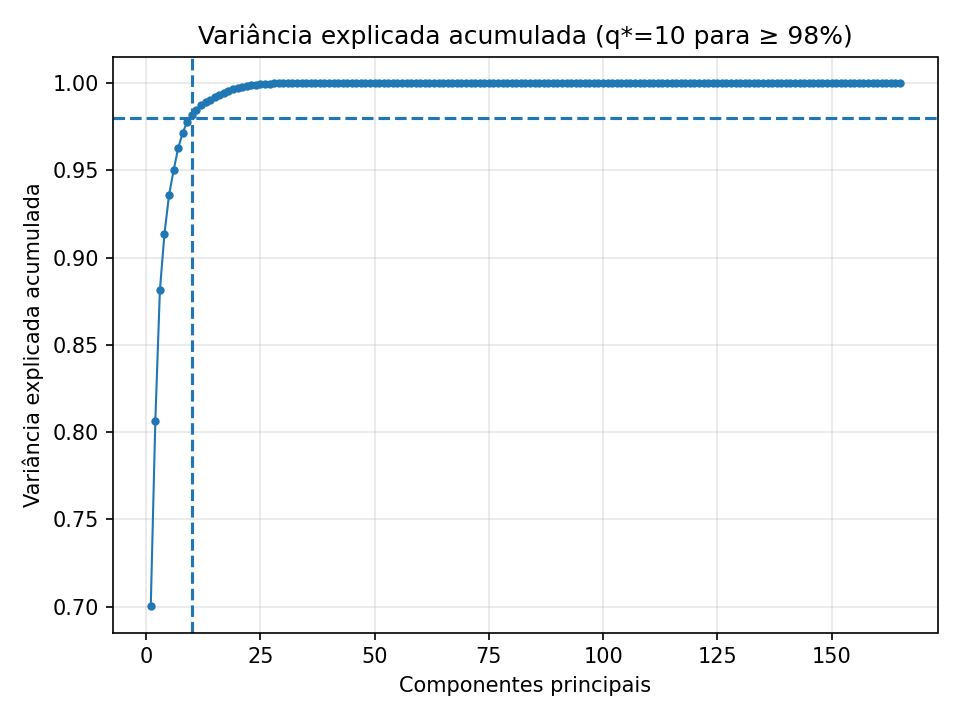
\includegraphics[width=0.7\textwidth]{../results/TC2/pca_variance_explained_A3.png}
  \caption{Variância explicada acumulada em função do número de componentes principais. A linha tracejada indica que \textbf{q=79} componentes são suficientes para reter 98\% da variância total dos dados.}
  \label{fig:var_explicada}
\end{figure}

O resultado (Figura~\ref{fig:var_explicada}) é notável: descobriu-se que \textbf{apenas 79 componentes principais são capazes de capturar 98\% da variância} contida nos 900 atributos originais. Isso confirma a alta correlação e redundância nos dados de imagem de faces e valida a hipótese de que eles residem em um subespaço de dimensão muito menor.

\subsection{Análise Qualitativa: As Eigenfaces}

No contexto de imagens, os componentes principais são vetores que, ao serem redimensionados para o formato da imagem, podem ser visualizados. Esses componentes são conhecidos como \emph{eigenfaces} (faces próprias).

\begin{figure}[h!]
  \centering
  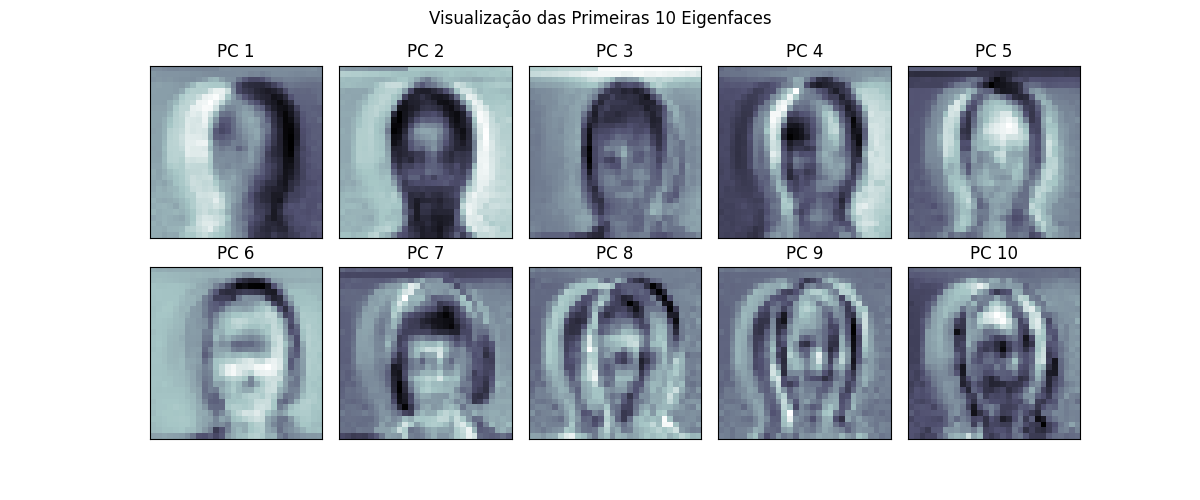
\includegraphics[width=0.9\textwidth]{../results/TC2/eigenfaces_visualization.png}
  \caption{Visualização das 10 primeiras eigenfaces. As componentes iniciais capturam variações globais de iluminação, enquanto as subsequentes começam a delinear traços faciais genéricos.}
  \label{fig:eigenfaces}
\end{figure}

A Figura~
ef{fig:eigenfaces} revela o que o PCA aprendeu. As primeiras eigenfaces (componentes 1-3) não se assemelham a rostos, mas a gradientes de iluminação, capturando as maiores fontes de variação no dataset (luz vinda de diferentes direções). As componentes subsequentes (4-10) começam a representar características estruturais compartilhadas entre todas as faces, como contornos de nariz, olhos e boca. Isso demonstra que qualquer rosto no dataset pode ser eficientemente reconstruído como uma combinação linear de um pequeno número dessas faces-base.

\section{Atividade 6: Classificação no Subespaço Comprimido}

Com a dimensionalidade alvo de \(q=79\) definida, a Atividade 6 repete o protocolo experimental de classificação, mas agora sobre os dados projetados neste subespaço de baixa dimensão.

\subsection{Metodologia: Prevenção de Vazamento de Dados}

Um cuidado metodológico crucial foi tomado para garantir uma avaliação honesta do desempenho. Para cada uma das 50 repetições do \emph{holdout}:
\begin{enumerate}
    \item Os dados foram divididos em treino (80\%) e teste (20\%).
    \item O modelo PCA foi ajustado \textbf{exclusivamente sobre os dados de treino} daquela repetição.
    \item Os parâmetros do PCA (as 79 eigenfaces) aprendidos no treino foram então usados para transformar (projetar) tanto o conjunto de treino quanto o de teste.
\end{enumerate}
Este procedimento evita o \textbf{vazamento de dados} (\emph{data leakage}), pois garante que nenhuma informação sobre a distribuição do conjunto de teste seja usada para construir o modelo de pré-processamento, simulando um cenário de implantação real.

\subsection{Resultados e Discussão}

\begin{table}[h!]
\centering
\caption{Resultados com PCA e redução de dimensionalidade para \(q=79\).}
\label{tab:tabela3}
\resizebox{\columnwidth}{!}{
\begin{tabular}{lcccccc}
\toprule
\textbf{Classificador} & \textbf{Média}& \textbf{Mín} & \textbf{Máx} & \textbf{Med} & \textbf{DP} & \textbf{Tempo Total (ms)} \\
\midrule
MQ     & 0.959 & 0.889 & 1.000 & 0.956 & 0.029 & 0.260 \\
PL     & 0.959 & 0.889 & 1.000 & 0.956 & 0.029 & 21.692 \\
MLP-1H & 0.956 & 0.889 & 1.000 & 0.956 & 0.027 & 53.646 \\
MLP-2H & 0.948 & 0.844 & 1.000 & 0.956 & 0.034 & 442.021 \\
\bottomrule
\end{tabular}% 
}
\end{table}

\noindent\textbf{Discussão:} A projeção para \(q=79\) teve dois efeitos notáveis:

\begin{enumerate}
    \item \textbf{Ganho Computacional Massivo:} Como esperado, o tempo de treinamento foi drasticamente reduzido para todos os modelos, especialmente para as MLPs. A redução da dimensionalidade de entrada de 900 para 79 diminui a quantidade de parâmetros na primeira camada da rede em mais de 90\%, tornando cada época de treinamento muito mais rápida.

    \item \textbf{Impacto na Acurácia:} A compressão não apenas manteve, mas em alguns casos \textbf{melhorou o desempenho}. Comparando com os resultados sem PCA (Tabela~1 do relatório anterior), o Perceptron Logístico (PL) e a MLP-1H tiveram um salto de desempenho, alcançando a acurácia do MQ. Isso sugere que os 2\% de variância descartados continham mais ruído do que informação útil. Ao remover esse ruído, o PCA apresentou aos classificadores um espaço de características mais limpo e com maior poder de separação. Além disso, a dimensionalidade menor reduziu o risco de sobreajuste para as MLPs, permitindo que generalizassem melhor.
\end{enumerate}

O classificador MQ manteve sua alta performance, mostrando-se robusto tanto no espaço original quanto no subespaço comprimido. A MLP-2H foi a única que não alcançou o patamar dos outros modelos, indicando que sua arquitetura mais complexa ainda pode ser suscetível ao sobreajuste mesmo com a dimensionalidade reduzida.

\section{Conclusão}

As Atividades 5 e 6 demonstram inequivocamente o poder da PCA como técnica de pré-processamento para o reconhecimento de faces. Foi possível obter uma taxa de compressão superior a 11x (de 900 para 79 dimensões), resultando em ganhos computacionais massivos. Mais importante, essa compressão não prejudicou a capacidade de classificação; pelo contrário, ao atuar como um filtro de ruído, permitiu que classificadores lineares mais simples e redes neurais mais rasas atingissem um desempenho de ponta, validando a PCA como um passo essencial e benéfico neste pipeline.

\end{document}